\chapter{The Model--View--Controller Pattern}
\label{chap:mvc}
This chapter discusses the \acl{mvc} pattern. It introduces design patterns in general, the classical \acl{mvc} architecture and different interpretations and variations of it.
\section{Design Patterns in Software Engineering}
The principle of using design patterns was first introduced by \citeasnoun{alexander}. The architects describe how a community can shape towns, neighbourhoods and buildings with simple tools. To communicate architectural knowledge in an effective way to the readers, he introduces \emph{design patterns}:
\begin{quote}
	\enquote{Each pattern describes a problem which occurs over and over again in our environment, and then describes the core to the solution to that problem, in such a way that you can use this solution a million times over, without ever doing it the same way twice.} \cite[p. 10]{alexander}
\end{quote}
This shows the main aspects of a design pattern:
\begin{enumerate}
	\item A pattern provides a solution to a specific, frequently occurring problem
	\item The pattern's solution is generic (only ``the core to the solution'', but no implementation details)
	\item The main advantage of a pattern is reusability
\end{enumerate}
Design patterns are a method of communicating solutions that have proven to solve a specific problem. Alexander's definition is open enough to be applied to nearly any field that deals with design problems, for example graphic design, architecture, interaction design, and software design. Most of these areas have repositories of design patterns. For architecture, there is the aforementioned book by Christopher Alexander, interaction design patterns can be found at the \emph{Yahoo! Design Pattern Library}\footnote{See \url{http://developer.yahoo.com/ypatterns/}}, and software design patterns are listed in the \emph{Portland Pattern Repository}\footnote{See \url{http://c2.com/ppr/}}.

\citeasnoun{gof} describe design patterns that are used in object-oriented software development. There are design patterns for other programming paradigms, but most of the more popular ones are created for object-orientation, especially as they leverage the given reusability that \acs{oop} provides through classes, interfaces, \glspl{prototype} or \glspl{mixin}.

Design Patterns simplify software development. If a pattern used in a software is well documented and understood, it is easier to maintain the software, to reuse code, and easier to communicate software architecture to new developers.

Gamma et al. classify the described design patterns into three categories, depending on their purpose.

\begin{description}
	\item[Creational Patterns] provide a way to create objects under certain circumstances (also known as \emph{object instantiation}).
	A popular example of creational patterns is the \emph{Singleton}, which ensures that only one instance of an object exists at a given time.
	\item[Structural Patterns] describe the composition (or \emph{structure}) of different objects or classes. They offer additional ways of composing as those already given through object-orientation (such as composition, aggregation or association). An example for a structural pattern is the \emph{Proxy}, which simulates the existence of a remote or otherwise unaccessible object by copying its interface and forwarding method calls. Amongst other purposes, proxies are used to simplify remote access or to realize access control.
	\item[Behavioral Patterns] are used to define the interaction of objects or classes, the flow of control or the distribution of responsibility. The \emph{Chain of Responsibility}, for example, is a sequence of interconnected objects that handle specific input. Depending on the type and content of this input, an element in the Chain of Responsibility may or may not process the input and pass it on to its successor.
\end{description}
According to \citeasnoun{gof}, design patterns exist on different levels of abstraction. The patterns described in \booktitle{Design Patterns} are mostly scoped on classes and objects. On a higher level of abstraction, there are \textbf{Architectural Patterns}\footnote{There are patterns of software architecture, not to be confused with the architecture patterns that \citeasnoun{alexander} described.}, one of them being \emph{\acl{mvc}}. Architectural patterns are not described by Gamma et al., but MVC in particular is mentioned as an illustrative example in the introductory chapter \citeyear[p. 4--6]{gof}. A collection of architectural patterns is listed by \citeasnoun{poeaa}.

%- Patterns are important to structure software
% compound: includes other patterns, such as publish-subscribe
% much interpreted, much misinterpreted
\section{History and Interpretation of MVC}
This section outlines the structure and control flow of \acl{mvc}. It explains the origins of MVC, describes the different components and discusses what leads to the different interpretations and variations of MVC.

\subsection{Origins of MVC in Smalltalk-80}
\acl{mvc} was first introduced by Trygve Reenskaug while he was working with the \gls{smalltalk} group at Xerox PARC from 1978 to 1979. He designed several versions that included the components ``Editor'' and ``Thing''\footnote{Editor and Thing are components that were part of very early versions of \ac{mvc}. They are not further discussed here.} before he settled on the MVC terminology. Reenskaug defined the MVC pattern for the use in applications with a \ac{gui}. His initial idea was to map the user's mental model of the data to the computational representation of the data. For this to achieve, he wanted to abstract the data, using different components and hiding the real Model from the user --- a principle that is called \emph{Separated Presentation}. Reenskaug summarized his work on \gls{mvc} in \booktitle{The Model--View--Controller (MVC). Its Past and Present}~\citeyear{reenskaug03}.

According to \citeasnoun[p. 99ff.]{osmani}, MVC takes the separation one step further and makes a clear division between the user interface and the application logic. This concept is now called --- more generally --- \emph{Separation of Concerns}. Before Smalltalk-80 MVC, Graphical User Interfaces were designed as one single module of code. This module handled the data, the presentation and the user interaction. While this worked well for tiny applications, it was hard to maintain for regular or large applications. Separating the presentation, user interaction (logic) and data allows to reuse these components.

\subsection{MVC Components}
Model, View and Controller are the components of a MVC architecture. Due to the high interpretability of this pattern, a common definition of the components and the pattern structure could not be found during research for this thesis. Thus, the definitions below are based on the different sources of Trygve Reenskaug, Gamma et al. and Martin Fowler.

\subsubsection{The Model}
MVC-based applications are data-centric, which means they are based on \emph{knowledge} that is organized in one or more \emph{Models}. A Model is the programmatic representation of these data, either the whole set or only a part.

Neither the characteristics of the data nor the way they are stored within the Model is relevant in this context. Data may be
\begin{itemize}
	\item \emph{structured}, such as a numerical table or a filled-out form
	\item \emph{semi-structured}, such as a XML or Microsoft Word document
	\item \emph{unstructured}, such as the body of an e-mail (free-form text).
\end{itemize}
A Model may store a particular element of its data in any way, depending on the data characteristics, the programming paradigm used and the requirements of the application. Possible storage models include, but are not restricted to
\begin{itemize}
	\item \emph{Objects} as used in object-oriented programming languages, such as Java objects or JavaScript objects
	\item \emph{Arrays} and \emph{Lists} as used in most programming languages
	\item \emph{Plain binary or textual streams} like files. A file system along with I/O functions can act as a Model.
\end{itemize}
Reenskaug described the original \ac{mvc} assuming Models would be Smalltalk objects, but with the spread of other programming languages and databases, every storage model can be imagined.

Often, Models contain more than just the plain data they embody. As is stated in \citeasnoun{reenskaug79a}, a Model is ``represented in the computer as a collection of data together with the methods necessary to process these data.'' This means, a Model can also contain functions, such as to \emph{create}, \emph{read}, \emph{update} and \emph{delete} data (also knows as \emph{\acs{crud}}). Auxiliary structures, such as hashes and indices, as well as functions add data-related business logic to the Model. They can simplify the handling of data extremely, for example through input validation, data conversion, sorting capabilities and faster access. % sollte business logic nur im controller sein? quelle?

A concept found in many collections of data, such as Java objects or relational databases, is the dependance of data on other data. A Java object, for example, can have the reference to a different object as one of its attribute values. In relational databases, a \gls{tuple} can refer to another tuple, which is part of either the same or a different \gls{relation}, using a foreign key. Those references have to be considered when designing Models.

In many cases, the data source is not the actual Model, depending on the point of view. If a Java application implementing \acl{mvc} needs to access data in a relational database, this is most probably implemented using an object-relational wrapper. From the point of view of the Java application, the wrapper classes are Models, while from an architectural point of view, the database (or the database tier) represents the Models. Such ambiguities lead to the need of good communication in the design and development teams, and they are one reason for the various interpretations of the pattern.

To clarify what the ``Model'' means in a given context --- for example, in one development team --- \citeasnoun{reenskaug79a} proposes that all Models should have the same level of abstraction. That means, ``Model'' should never describe a database and, at the same time, an object holding data from this database, which would be more concrete than the database itself and thus on a different level of abstraction.

\subsubsection{The View}
As MVC is a pattern for applications with a user interface, the View is responsible for (visual) data presentation. It can reach from a simple, textual representation to tables, charts and diagrams or even more complex output. A View is always connected to a Model and is used to present the Model's data. A View is usually related to one Model only, whereas a Model can have multiple Views.

The output medium according to \citeasnoun{reenskaug79a} is either the screen or hardcopy (print), but nowadays other output media, such as audio (for example a speech synthesizer) or haptics (for example a \emph{braille} device used by blind people to interact with a computer) can be applied to the View concept. However, in software development, the screen is still the main output device, and is focused on in this definition; therefore, the terms ``present'', ``show'' and ``display'' are used synonymously.

Usually, not all data of a Model are presented at once. There are two ways of limiting the presented data, both of which can be compared to relational algebra for illustration. On the one hand, a View can display only several chosen facets of the Model. This can be compared to a \emph{projection} in relational algebra. On the other hand, the set of data can be limited, so that only items that match certain criteria or not more than a specific number of items are displayed. This can be compared to a \emph{selection} in relational algebra.

As the View is an interface to the user, the functionality described above is needed in order to let the user focus on the important part of the data. Scrolling, pagination and lazy loading are all examples for features that support this functionality of the View component. \citeasnoun{reenskaug79b} calls the View a ``presentation filter''.

To fulfill the task of presenting a Model's data, a View has to know about the Model. (In contrast, the Model is totally independent of the View.) This knowledge is needed for two reasons: On the one hand, it needs to have access to the actual data to be able to display them. On the other hand, a View may need to know metadata to display the actual data properly.

To illustrate the latter, we can imagine a table (View) that displays data from a relational database (Model). Whereas some columns show text or numbers, another one displays dates which have to be formatted according to the user's local settings. This cannot be the Model's task; it is aware of the fact that this piece of data is a date, but it does not know how to format a date properly. This would be the task of the presentation component, which in \acl{mvc} is the View.

The data a View displays are held in the View's private buffer. When the Model changes, the View has to be informed about that to update these data. To fulfill this, the View is connected to the Model via an Observer pattern as described by \citeasnoun{gof} (see Section~\ref{sec:modelview} for more information on the Observer).

\subsubsection{The Controller}
The exact role of the Controller is probably the most discussed part of \acl{mvc}. The resulting variations, such as \acl{mvvm} or \acl{mvp} all kept the Model and View, but redefined what used to be the Controller. To clearly draw a picture of the Controller's task, Reenskaug's definition is taken into account:
\begin{quote}
	\enquote{A controller is the link between a user and the system. It provides the user with input by
	arranging for relevant views to present themselves in appropriate places on the screen. It
	provides means for user output by presenting the user with menus or other means of giving
	commands and data. The controller receives such user output, translates it into the appropriate
	messages and pass these messages on to one or more of the views.} \cite{reenskaug79b}
\end{quote}
In other words, the Controller is the part of an application that implements the overall application flow and the user interaction. As already mentioned, \acl{mvc} is an architectural pattern for applications with a \acl{gui}. The Controller processes user input, for example such input that is used to manipulate the Model.

Some interpretations add the term of an \emph{Application Controller} to pay respect to the fact that there are Controllers on different layers of the application, as described by \citeasnoun[pp. 379--386]{poeaa}. A View-bound Controller may react when the View is clicked, but it can only know that from a higher--level Application Controller that tracks mouse movements and events. In the case of web applications, this is the browser (or the JavaScript engine, respectively). According to \citeasnoun{fowlergui}, there is ``not just one view and controller, you have a view-controller pair for each element of the screen, each of the controls and the screen as a whole.''

The term \emph{Front Controller}\label{term:frontcontroller} describes an object that manages the application state and navigation by providing a single entry point to the application\footnote{The Front Controller is called \emph{Router} by \citeasnoun{osmani}.}. In the area of web pages, a Front Controller is a ``A controller that handles all requests for a Web site.'' according to \citeasnoun[p. 344]{poeaa}. One example for such a Controller is the Servlet employed in \emph{Model 2}, a Java EE MVC architecture using JSPs, EJBs and Servlets (see Section~\ref{sec:thinclient}).

\subsection{Model, View and Controller in Interaction}
The separation of data, presentation and interaction is a powerful way to structure an application. The goal of MVC is reusability and maintainability, but the three components still have to work together to make sense. The introductory chapter of \booktitle{Design Patterns} describes the different design patterns used within MVC~\cite[pp. 4--6]{gof}.

\begin{figure}[H]
	\centering
	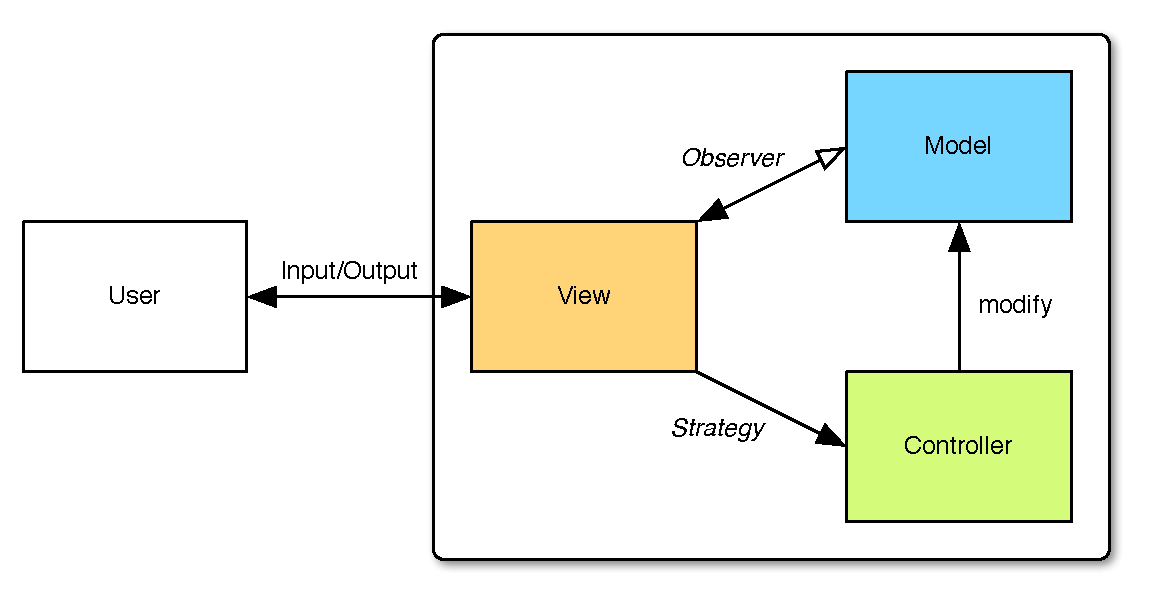
\includegraphics[width=12cm]{images/mvc.pdf}
	\caption{Structure of \acl{mvc}}
	\label{fig:mvc}
\end{figure}



\subsubsection{Model and View}
\label{sec:modelview}
According to \citeasnoun[p. 4]{gof}, ``MVC decouples views and models by establishing a subscribe/notify protocol between them.'' In other words, the View ``subscribes'' to the Model, and the Model then notifies the View whenever the Model's data change. Eventually, the View can update itself to reflect those changes. The \emph{subscribe/notify} solution described by the \emph{Observer} pattern in \citeasnoun[pp. 293--303]{gof} is also called ``Publish--Subscribe'' and allows multiple Views to observe a single Model (see Figure~\ref{fig:modelview}).

\begin{figure}[H]
	\centering
	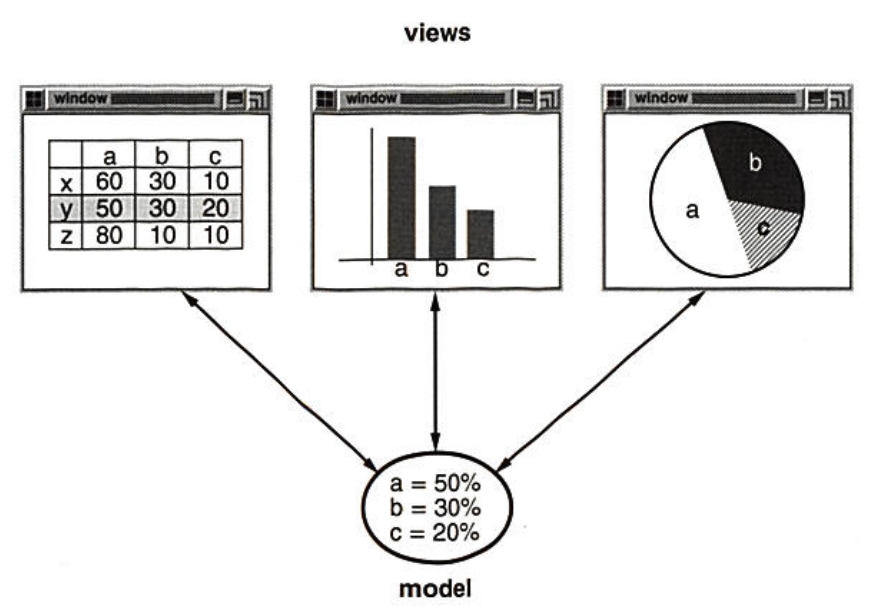
\includegraphics[width=12cm]{images/modelviewhd.png}
	\caption{Multiple Views connected to a single Model}
	\captionsetup{font={footnotesize,bf,it}}
	\caption*{Source: \citeasnoun[p. 5]{gof}}
	\label{fig:modelview}
\end{figure}

According to \citeasnoun[p. 108]{osmani}, the ``observer nature of this relationship is what facilitates multiple views being attached to the same model.'' This means that Model and View are completely decoupled. The Model does not know about the View, it only notifies all its subscribers when it changes. A subscriber can be any arbitrary object, which only needs to implement a special function to receive the notification (in Java, this is typically realized using an \emph{interface}). Thus, a subscriber does not even have to be a View, which means that the Model is completely isolated from the \ac{ui} part of the application (if there is any).

\subsubsection{View and Controller}
The relationship between View and Controller is defined by a Strategy pattern, or in other words: the View uses the Controller as a Strategy object. A Strategy object is an object representing an algorithm. If an interaction is triggered on the View, for example a key press, mouse movement or mouse click, the View recognizes it and invokes the Controller. The Controller then decides on how to react to the according event.

A good example is \emph{scrolling} in a scrollable list. This list (the View) is constrained in its height, so it can only display a part of the list items. List items are stored in the Model. As soon as the user initiates scrolling, for example by moving the mouse wheel or moving the scoll bar, the View calls the Controller. The Controller recognizes the event as scrolling and calls back the View to update itself. Depending on how far the user scrolled, other list items are shown in the list. This course of events is also illustrated in Figure~\ref{fig:seqmvc}.

On his website, \citename{reenskaugweb} describes the pair of View and Controller as the \emph{Tool} (see Figure~\ref{fig:tool}). But, as the Gang of Four writes in \booktitle{Design Patterns: Elements of Reusable Object-Oriented Software}, it is important to keep this coupling loose. This allows a software developer to easily replace a View's Controller, even at runtime, to change its interactive behaviour. The example from \citeasnoun[p. 6]{gof} proposes that, to disable interaction on a View, one could assign to it a Controller that ignores any interaction.
\begin{figure}[H]
	\centering
	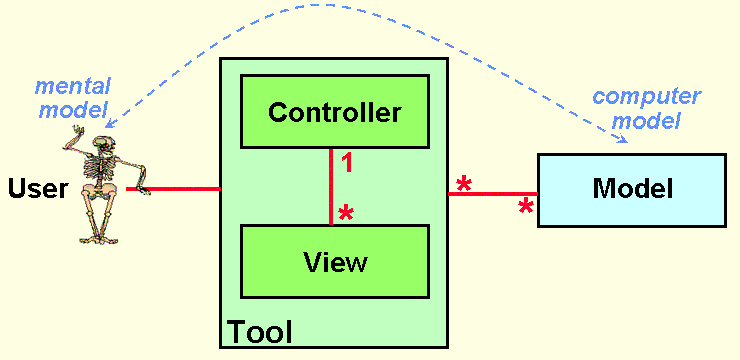
\includegraphics[width=12cm]{images/MVC-2006.png}
	\caption{The Tool contains Controller and View(s)}
	\captionsetup{font={footnotesize,bf,it}}
	\caption*{Source: \citeasnoun{reenskaugweb}}
	\label{fig:tool}
\end{figure}

\subsubsection{Controller and Model}
As described above, one task of the Controller is to react to the user's input. When the user's interaction is targeted at manipulating the domain data, for example by changing the value of a table cell, the Controller's task is to update the Model accordingly.

As mentioned by \citeasnoun[pp. 105, 108]{osmani} and \citeasnoun{reenskaug79b}, the Controller updates the View after the Model changes, but this is not necessary in implementations where the View observes the Model, as is stated in \citeasnoun{fowlergui}: ``When the model changes, the views react.'' The sequence diagram of \emph{Figure 6: Changing the actual value for MVC.} by \citeasnoun{fowlergui} emphasizes that (see Appendix). Subsequently, Addy Osmani clarified that it is ``absolutely correct that the Observer relationship should be responsible for updating the View. The Controller should in no way be changing the View directly.''\footnote{Personal conversation with the author, 07/23/2012}

%The relationship of Controller and Model is unidirectional: the Model does not know about the Controller. In some implementations, the Model might know a Controller via the Observer relationship of View and Model, but as a Controller can also change Models that are not directly associated with its respective View, this is not alway the case.

As it can be seen, the role of the Controller is subject to very different interpretations.

\subsubsection{Flow of Control}
\label{sec:flowofcontrol}
The View and Controller are defined as two very separate objects, the View being responsible for presentation (output), the Controller being responsible for user action (input). It is a matter of definition if a user interaction is performed \emph{on the Controller}, or if it is performed \emph{on the View} and the View then uses the Controller to react to it (\emph{Strategy} pattern). The first variant is illustrated by \citeasnoun{fowlergui} in the sequence diagram of \emph{Figure 6: Changing the actual value for MVC} (see Appendix) as well as by \citeasnoun{steele}. Some sources, however, assume the latter case (the \emph{Strategy} pattern), as it is described in \citeasnoun[p. 6]{gof}. In this thesis, both variants are taken into account, depending on which one makes more sense in a given situation.
\begin{figure}[H]
	\centering
	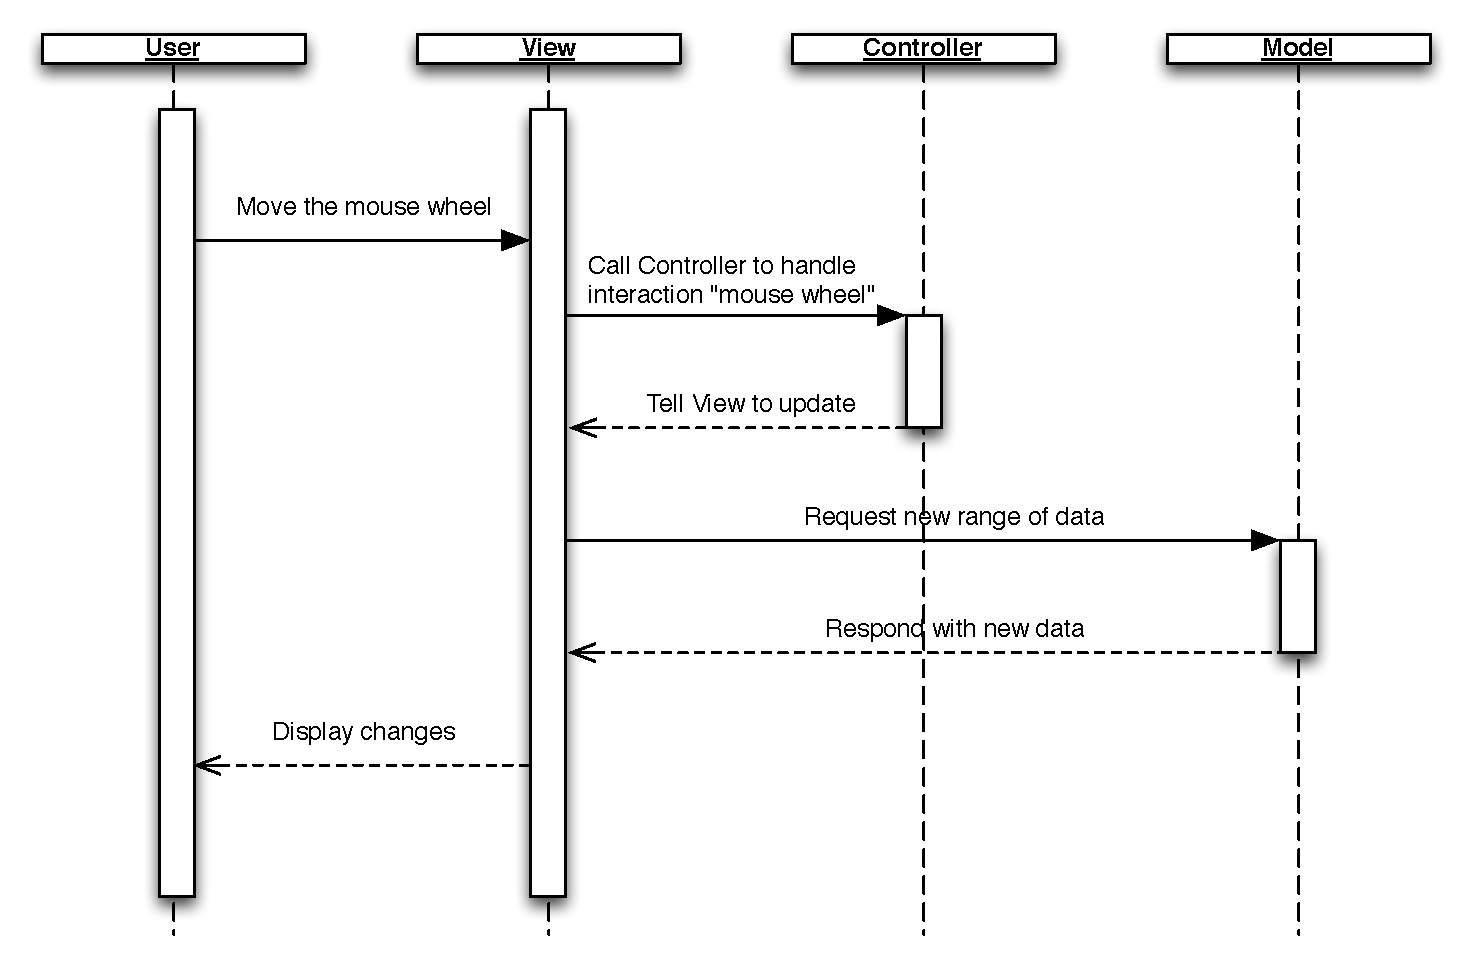
\includegraphics[width=16cm]{images/seqmvc.pdf}
	\caption{Sequence diagram of a User Interaction with \acl{mvc}}
	\label{fig:seqmvc}
\end{figure}
The sequence diagram in Figure~\ref{fig:seqmvc} illustrates the user scrolling over a list of items.

\section{Pattern Variations}
The following section describes variations of MVC that can be found in modern software architecture, especially in web applications and the according frameworks. Those variations are an answer to the different interpretations of \acl{mvc}, primarily regarding the responsibilities of the components. \gls{mvc} and its variations are often called the \emph{MV* family} of patterns \cite{osmani}.

\subsection{Model--View--Presenter}
The first variation of \ac{mvc} to be discussed is \ac{mvp}. It was created in the early 1990s to improve presentation logic for the \gls{Taligent} operating system and has been adapted in a slightly modified form for the use in web applications by the \emph{Backbone.js} framework\footnote{See \url{http://backbonejs.org/}}.

The Model in \ac{mvp} behaves similar to the one of \ac{mvc}: it contains and handles domain data. The difference to \ac{mvc} is in the View and the \emph{Presenter} which replaces the Controller.

The \ac{mvp} View is called a \emph{Passive View}, because it contains as few logic as possible (thus being ``dumb''), as described by \citeasnoun{fowlerpv}.

The Presenter, however, has additional responsibilities compared to the Controller. In Smalltalk-80 \ac{mvc}, the View gets the data to display directly from the Model. In \ac{mvp}, the Presenter separates this connection, acting as a mediator between the View and the Model \cite[p. 109]{osmani}. It decouples Model and View completely by breaking up the Observer connection. The original Controller tasks of manipulating the Model and processing user input are in the responsibility of the Presenter, too.

There are two exceptional advantages in combining the Presenter as a mediator with the Passive View, according to \citeasnoun{osmani} and \citeasnoun{fowlerpv}:
\begin{itemize}
	\item It allows developers to rapidly prototype user interfaces. Most of the presentation and business logic (which is not relevant in the context of prototyping) is in the Presenter, whereas the View is the component being prototyped.
	\item The thin presentation layer embodied by the Passive View makes automated testing possible, which in other cases is hard to do with a user interface.
\end{itemize}

Due to the Passive View, View and Presenter are completely decoupled in MVP. There is no data-binding of the View to the Presenter. This means, it is up to the Presenter to decide how to display data in the View, whereas in other implementations (MVC, MVVM) the View contains the presentation logic.

\begin{figure}[H]
	\centering
	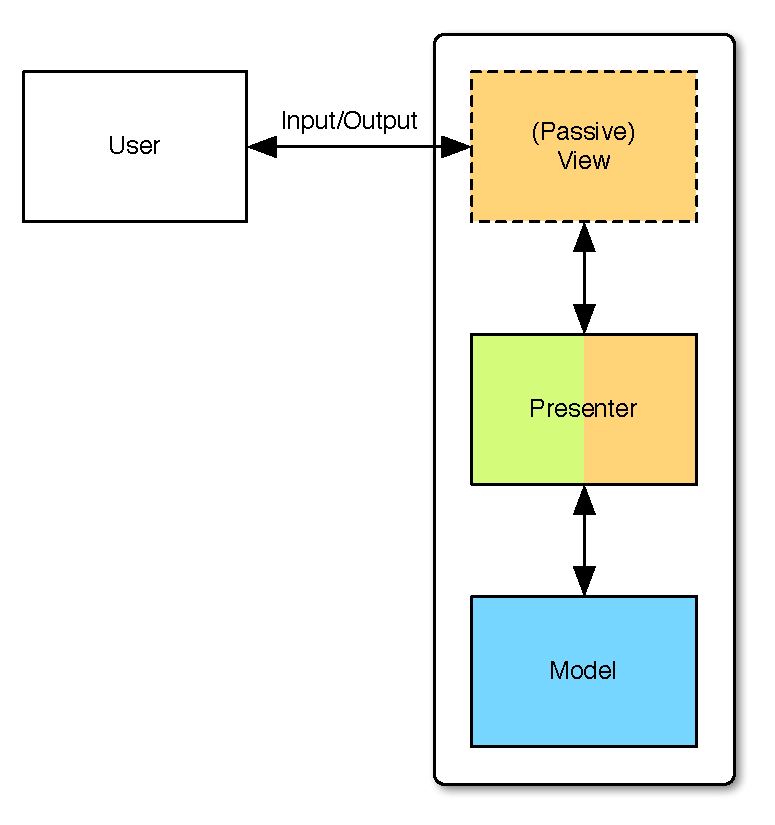
\includegraphics[width=8cm]{images/mvp.pdf}
	\caption{Structure of \acl{mvp}}
	\label{fig:mvp}
\end{figure}

\subsection{Model--View--ViewModel}
A second variation of MVC widely used in web applications is \ac{mvvm}. It was first introduced with Microsoft Silverlight\footnote{Silverlight is a browser extension to include rich media, similar to Adobe Flash.} in 2007. \citeasnoun{poeaa} describes a similar pattern, called ``Presentation Model''. MVVM is based on MVC and MVP and includes concepts of both.

Just as in MVC and MVP, the Model contains domain data and the according CRUD functinality.

In opposition to MVP, the MVVM View is not passive. It contains presentation logic and decides if and when to update itself. In MVP, this task is done by the Presenter. The Presenter ``pushes'' changes of the Model to the View, whereas the ViewModel only ``notifies'' the View of those changes; it is up to the View to request the changed data and format them to its purpose.

The term ``ViewModel'' is caused by this component acting like a View-specific Model. Just like the Presenter in MVP does, it decouples the View from the Model and acts as a mediator between them. The difference to a Presenter is, that the ViewModel handles data modelling rather than presentation. It listens for changes in both the Model and the View and synchronizes them, doing only basic data conversions\footnote{For example, the conversion from a UNIX timestamp (``1342177280'') to a localized timestamp (``July 13, 2012 11:01:20'').}.

ViewModel and View are connected through bidirectional data bindings, which act as the single interface between these two components. In its relationship to the View, the ViewModel can be compared to the MVC Model, which also notifies the View of changes, but does not change the View directly.

From a high level point of view, the structures of MVVM and MVP are the same. The differences are in the responsibilities and the coupling of the components; Figure~\ref{fig:mvp} and Figure~\ref{fig:mvvm} illustrate this using colors representing the responsibilities of the MVC components, which are differently distributed in MVP and MVVM.

\begin{figure}[H]
	\centering
	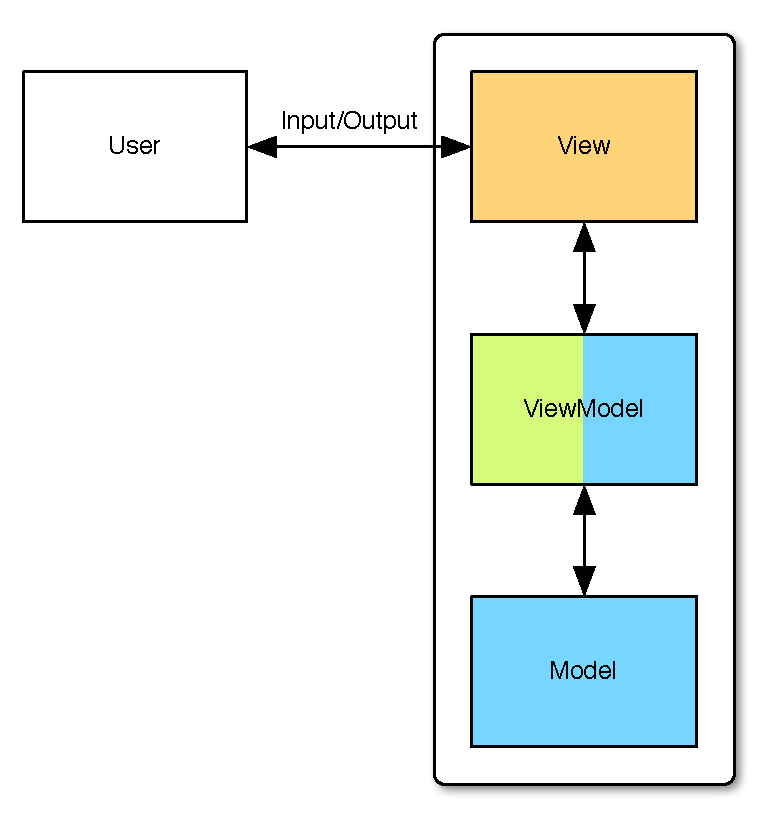
\includegraphics[width=8cm]{images/mvvm.pdf}
	\caption{Structure of \acl{mvvm}}
	\label{fig:mvvm}
\end{figure}


\subsection{Comparison of MVC, MVP and MVVM}
The following example illustrates the differences between MVC, MVVM and MVP: A part of an application displays a list of tasks. In the Model, they are organized as an array of task objects, each of which has different attributes, such as the task name, the due date and the state (``done'' or ``not done''). There are a hundred tasks, but the UI has to display only the first ten tasks.

In MVC, the View fetches the data it needs (the first ten items) directly from the Model. As the View already is a list presentation, it only needs to add the tasks as list items. The Controller is not involved in this process.

In MVP, the Presenter fetches the items it needs (the first ten) from the Model. It then formats them as a list with every list item having a check box next to it. This list gets forwarded to the View and is displayed there.

In MVVM, the View tells the ViewModel that it needs the first ten task items. The ViewModel then fetches those items from the Model and send them to the View. The View formats them as a list.

Basically, all three patterns fulfill the same tasks. As mentioned before, the difference is in the responsibilities of the various components.

The MVVM View contains more presentation logic than the MVP one, its structure is given and it prepares the data for presentation itself (except for logical conversions). In MVP, this is the Presenter's task, while the View keeps passive.

Both MVP and MVVM decouple the Model from the View, in opposition to MVC. The direct access from the View to the whole Model in MVC is considered bad by \citeasnoun[p. 123]{osmani}, as it can ``have security and performance costs''. In other words, access to the Model is neither controlled nor cached. The missing ability to cache data in MVC may be a downside compared to MVP and MVVM, but on the other hand, there is less processing of data between View and Model. When data conversions in Presenter or ViewModel are complex, this can be an advantage for MVC.

It is a matter of preference and use case to choose the architectural pattern that suits an application best. In the following chapters, especially in Chapter~\ref{chap:webmvc}, MVC is assumed to be the pattern used, but the components marked as Model, View and Controller do not have to be distinct objects --- it is more important to understand that they fulfill the tasks and have the responsibilities of the respective MVC components, as described earlier in this chapter.